\chapter{Evaluation}
In this chapter, we firstly discuss the reason behind creating a new dataset. We further present achieved results with our proposed framework, and lastly, we propose additional improvements for future work.

\section{Dataset}
    There are many public annotated datasets \cite{MOTChallenge2015, ferryman2009pets2009, zhuvisdrone2018} for a person tracking task and many others targeting soft-biometrics \cite{goodfellow2013challenges, yang2016wider}. However, their focus is a little different than what is needed for the evaluation of this thesis. Firstly, individuals only appear in a few images of the sequence, which is not entirely the case for retail, where it is required to maintain the individual's long-term identity even in the case of multiple occlusions. Secondly, these datasets do not focus on the joint task of tracking and soft-biometrics extraction. The available tracking sequence lacks additional information about people and the scene parameters that are required to calibrate the camera. It was, therefore, advisable to create an in-the-wild dataset to simulate a real scenario.
    
    The 14th floor of the \gls{fce} \gls{ctu} building was used to create a dataset, where it was possible to place a camera to a place that is most similar to the retail case. In total, over 10,000 images were captured, of which 2463 frames were hand-annotated with person bounding-boxes and identities. There are a total of 7028 bounding boxes with 11 person identities. Face regions were not annotated because it would have no added value for the evaluation. Related individual's soft-biometrics data such as age, gender, and height are known, but ground-truth data for emotions and trajectories are not available. There are only male representatives in the dataset. Captured frames are not further pre-processed.
  
\section{Hardware and software setup}\label{evaluation_estup}
    The speed performance of algorithms is tightly dependent on the utilized hardware and software setup. The proposed methods were tested on the computer available in \gls{improlab}. The testing setup consisted of Intel~i5~-~7600K~@~3.80GHz, NVIDIA GeForce RTX 2080 TI, 16 GB RAM, and SSD disk. The software dependencies were CUDA 10, cuDNN 7.5, Tensorflow 1.13, OpenCV 3.4.2, and the latest version of Darknet. All third-party libraries were compiled for GPU support.

\section{Tracking results}
    In order to be able to compare individual tracking solutions among each other, it is necessary to determine a suitable metric. Because metrics for object detection and tracking in the video can often be non-intuitive and complex, the well-known \gls{motp} and \gls{mota} metrics are adopted in this work. \gls{motp} metrics focus on the quality of detected regions, while \gls{mota} focuses on tracking accuracy, and its calculation affects the number of \glsentryfull{fp}, \glsentryfull{fn}, and \glsentryfull{idsw}. Factors affecting \gls{mota} are also compared, as it is interesting to see how they change depending on the detection network. The metrics are described in more detail in section \ref{evaluation-metrics}; however, to be concise, higher \gls{mota} or \gls{motp} means better.
    
    We present our results in table \ref{table:tracking_results} for different object detection architectures -- \gls{yolo}v2, \gls{yolo}v3, \gls{yolo}v3 \gls{spp}, and \gls{faster r-cnn} with ResNet50 backbone. For the retail usage, the number of identity switches (\gls{idsw}) is a crucial metric, and in this aspect, the \gls{faster r-cnn} outperformed other detectors by a large margin. We also provide some output predictions in Fig. \ref{fig:examples_of_outputs} and example video in \cite{trackingvideo} demonstrating robustness of the proposed algorithms.  
    
    \begin{table}[h]
        \centering
        \begin{tabular}{|c|c|c|c|c|}
            \hline
            \rowcolor{Blue}
            \color{White}\textbf{} & \color{White}\textbf{\gls{yolo}v2} & \color{White}\textbf{\gls{yolo}v3} & \color{White}\textbf{\gls{yolo}v3 SPP} & \color{White}\textbf{\gls{faster r-cnn}} \\ \hline \hline
                \gls{motp} & 0.795 & 0.84 & 0.89 & 0.87 \\ \hline
                \gls{mota} & 0.825 & 0.94 & 0.905 & 0.94 \\ \hline
                \gls{fn} & 879 & 306 & 470 & 228 \\ \hline    
                \gls{fp} & 147 & 132 & 223 & 167 \\ \hline    
                \gls{idsw} & 14 & 8 & 10 & 2 \\ \hline
                \gls{fps}  & 26.62 & 22.2 & 16.29 & 17.37 \\ \hline    
        \end{tabular}
        \caption{Tracker evaluation table.}
        \label{table:tracking_results}
    \end{table}
    
    \begin{figure}[h]
        \centering
        \subfloat[]{{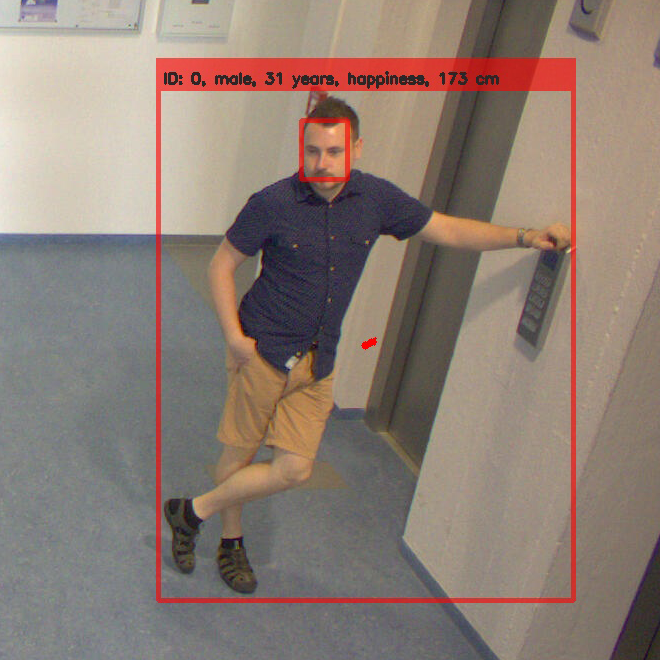
\includegraphics[width=0.28\textwidth]{resources/framework_example_1.png} }}
        \qquad
        \subfloat[]{{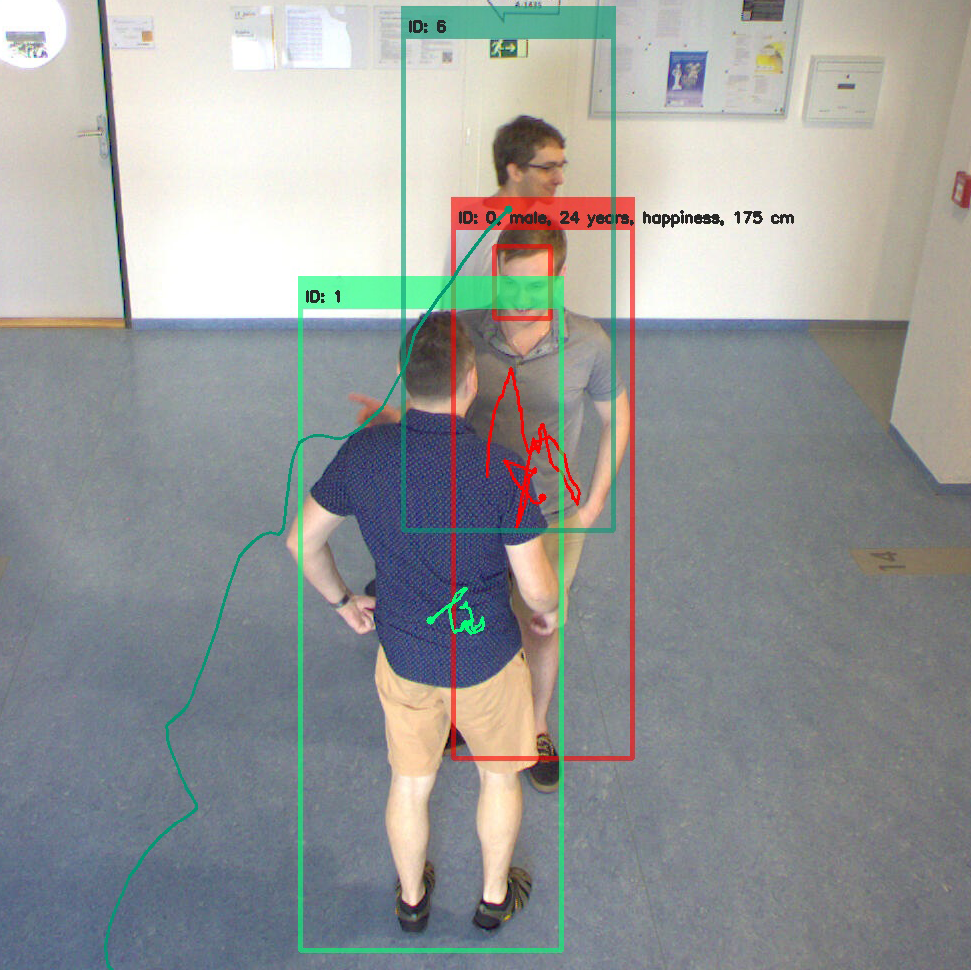
\includegraphics[width=0.28\textwidth]{resources/framework_example_2.png} }}
        \qquad
        \subfloat[]{{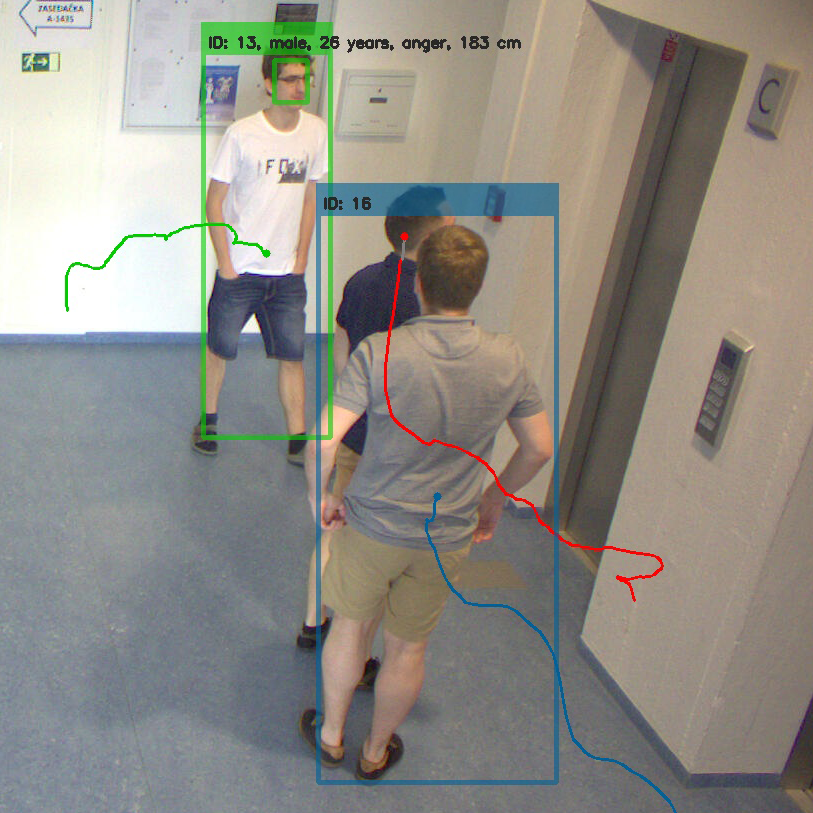
\includegraphics[width=0.28\textwidth]{resources/framework_example_3.png} }}
        \caption{Image examples of our framework. (a) An example of a person facing the camera so his biometrics can be accurately estimated. Only the height value is inaccurate by 2 cm, which is a very precise outcome. (b) An example of people who are close to each other without affecting the tracker accuracy. (c) An example of people who are even closer than in (b). The person in the middle is fully occluded, and no detection is available for him. However, the red circle is trying to predict his position, in case he reappears in the scene. The prediction of soft-biometrics for the person with ID 13 is inaccurate by one year and 3 cm.}
        \label{fig:examples_of_outputs}
    \end{figure}

    In the table with results, we can see that the more complex the architecture employed, the more accurate the results, which again verified the fact presented in the introduction chapter, that a robust object detector is a key to proper tracking. Specifically, we can observe the number of missed detections (\gls{fn}) and identity switches (\gls{idsw}) is decreasing with more robust architecture. \Gls{faster r-cnn} generally has more "ghost" detections (\gls{fp}), but it was something we expected already in the Methodology chapter, and it is not such a problem that would significantly affect the results of the framework. 
    
    Interesting observations are worse results achieved by the modified \gls{yolo}v3 with \glsentryfull{spp} architecture. According to the original paper, it should work better on small objects, and although it provided more accurate bounding boxes (\gls{motp}), all other aspects suggest that it is not very suitable for tracking algorithms.  
    
    The fact that FPS is decreasing with the complexity of object detector architecture is no surprise. Generally speaking, the bottle-neck of the tracker is the object detector. Based on our observations and measurements, the tracking algorithm without the object detector component can run at around 500 \gls{fps}. It is, therefore, necessary for any task to select the suitable object detector first. In our case, even with the complex \gls{faster r-cnn}, the tracking achieves near real-time performance.
    
\section{Soft-biometrics results}
    The evaluation of soft-biometrics is a bit more complicated. It is not possible to obtain precise ground-truth for trajectories and emotions, so there is no room for evaluation. However, three more remaining features could be possibly evaluated -- age, gender, and height. We decided to choose only age and height for the evaluation because we could not find a female representative at the time of the dataset creation. 
    
    The situation is even more complicated because some biometric information cannot always be extracted. It may happen that a person will always be back to the camera and it will not be possible to extract his facial information, or a person moves very fast or is occluded all the time, so it is not possible to estimate his height. Therefore, we only evaluate cases where it is possible to extract suitable soft-biometric data.
    
    We use \glsentryfull{mae} metric described in section \ref{evaluation-metrics} for evaluation instead of \gls{rmse} because it has easier interpretation. Description of the utilized detectors can be found in Methodology chapter. 
    
    In table \ref{table:age_estimation_results}, we present our outcome for age estimation for various face detectors. From the results, we can observe that the alignment feature in MTCNN has a great positive impact on accuracy, but it drastically reduces the \gls{fps}. Tensorflow Mobilenet \gls{ssd} architecture provides the best trade-off between performance (\gls{fps}) and accuracy (Age \gls{mae}).

    \begin{table}[h]
        \centering
        \begin{tabular}{|c|c|c|c|}
            \hline
            \rowcolor{Blue}
            \color{White}\textbf{} & \color{White}\textbf{faced} & \color{White}\textbf{Mobilenet \gls{ssd}} & \color{White}\textbf{MTCNN} \\ \hline \hline
                Age \gls{mae} & 5.21 & 3.82 & 2.65  \\ \hline
                \gls{fps} & 78.41 & 119.86 & 7.01 \\ \hline
        \end{tabular}
        \caption{Age estimation evaluation table.}
        \label{table:age_estimation_results}
    \end{table}

    The last table \ref{table:height_estimation_results} focuses on the influence of object detector on height estimation. \Gls{yolo} architectures generally provide less accurate bounding boxes, thus making the height error larger. The achieved results correspond to the \gls{motp} outcome in table \ref{table:tracking_results}. We can also see that the speed performance degradation compared to the original \gls{fps} is negligible. To conclude, height estimation works well in most cases, and it has a little computational overhead.
    
       \begin{table}[h]
        \centering
        \begin{tabular}{|c|c|c|c|}
            \hline
            \rowcolor{Blue}
            \color{White}\textbf{} & \color{White}\textbf{\gls{yolo}v2} & \color{White}\textbf{\gls{yolo}v3} & \color{White}\textbf{\gls{faster r-cnn}} \\ \hline \hline
                Height \gls{mae} & 7.31  & 5.84 & 4.09  \\ \hline
                \gls{fps} & 26.35  & 21.97 &  17.17 \\ \hline
        \end{tabular}
        \caption{Height estimation evaluation table.}
        \label{table:height_estimation_results}
    \end{table}
    
\section{Further work}
    This complicated and broad task is not something that can be fully accomplished in one final thesis. Therefore, in this section, we suggest some improvements for future work.
    
    \subsection{Tracking improvements}
        Current state-of-the-art object detectors are already achieving outstanding results. People are detected in most cases when they are visible. The problem arises when people are entirely occluded, so they are not visible to the camera, but we still need to retain their identity when they show up. This is a situation where having robust tracker helps. 
        
        Our tracker can deal with short-term occlusions which are mostly situation when people pass by. However, it is not designed for the case when individuals are completely missing for a few seconds. To improve in this manner, the missing tracks would need to be kept in the memory for a more extended period than 50 frames, but also a new matching metric for these cases would need to be developed.
        
        The tracking performance could also be improved by adding a non-linear state filter such as unscented Kalman filter or particle filter, which would improve the matching phase. The reason is that not all people behave linearly in their movement. Therefore, the current filter may occasionally diverge.

        From our observation, utilized object detectors are already robust with default parameters and pre-trained models. Therefore, there is no reason for re-training them for a particular task with people. There could be significant speed-up improvement by proposing an object detector that can detect faces and people simultaneously.

    \subsection{Soft-biometrics extraction improvements}
        Our framework can extract face information (age, gender, emotion), height, and trajectory. This information can only be obtained under certain conditions. If no face is visible during the whole tracking session, then it is not possible to output any face information. If the object moves quickly, then extracted height information is not accurate. Moreover, if an object is occluded, then trajectory information might contain gaps.
        
        Of course, all these shortcomings could be improved, but the significant improvement, for now, would be retraining the face extraction models on more in-the-wild data to improve the accuracy. There is no need to replace utilized architectures as they achieve state-of-the-art performance on current datasets, but it is needed to fine-tune the weights by faces that are captured at an angle, not only from the front view. It would also help to evaluate the methods on data from multiple environments and with more types of people.
        
        Another improvement could be achieved by employing a model that can do face embedding. This embedding then could be used in the matching phase to recover long term occluded individuals. 